\documentclass[tikz,border=10pt]{standalone}
\usepackage{tikz}
\usepackage{amsmath,amssymb}
\usetikzlibrary{arrows.meta,positioning,fit,backgrounds}

%% ── Color palette (print-safe, distinct in grayscale) ─────────────────────
\definecolor{cObs}    {RGB}{127,140,141}   % slate gray
\definecolor{cEnc}    {RGB}{ 41,128,185}   % cobalt blue
\definecolor{cEdge}   {RGB}{ 21, 92,147}   % deep blue
\definecolor{cGNN}    {RGB}{125, 60,152}   % violet
\definecolor{cSlot}   {RGB}{211, 84,  0}   % burnt orange
\definecolor{cCross}  {RGB}{ 39,174, 96}   % emerald
\definecolor{cGRU}    {RGB}{ 22,160,133}   % teal
\definecolor{cActor}  {RGB}{192, 57, 43}   % crimson
\definecolor{cCritic} {RGB}{150, 40, 27}   % dark crimson
\definecolor{cRobot}  {RGB}{ 44, 62, 80}   % dark navy
\definecolor{cAux}    {RGB}{230,126, 34}   % amber
\definecolor{bgP}     {RGB}{235,245,255}   % pale blue  — perception bg
\definecolor{bgN}     {RGB}{235,252,242}   % pale green — navigation bg
\definecolor{bgA}     {RGB}{255,248,230}   % pale amber — aux supervision bg

\begin{document}
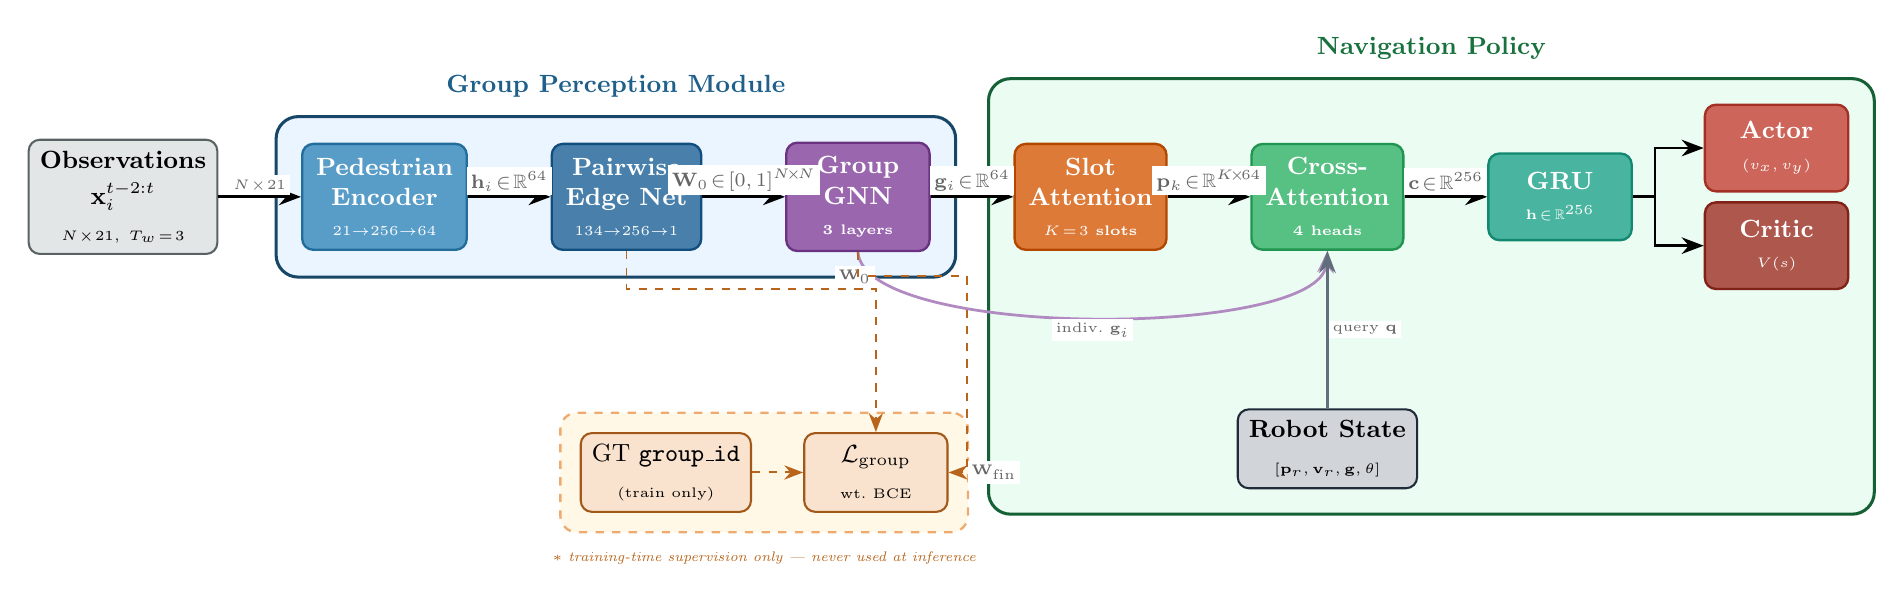
\begin{tikzpicture}[
  node distance = 0.5cm and 1.05cm,
  %% ── coloured stage block ──────────────────────────────────────────────
  S/.style={
    draw=#1!85!black, fill=#1!78,
    rounded corners=4pt, line width=0.85pt,
    minimum width=1.82cm, minimum height=1.10cm,
    align=center, font=\small\bfseries, text=white, inner sep=5pt
  },
  %% ── input / helper block ──────────────────────────────────────────────
  I/.style={
    draw=#1!70!black, fill=#1!22,
    rounded corners=4pt, line width=0.75pt,
    minimum width=1.82cm, minimum height=1.00cm,
    align=center, font=\small, inner sep=4pt
  },
  %% ── main arrow ────────────────────────────────────────────────────────
  A/.style={-{Stealth[length=2.8mm,width=2.1mm]}, line width=1.0pt},
  %% ── auxiliary (dashed) arrow ──────────────────────────────────────────
  D/.style={-{Stealth[length=2.4mm,width=1.8mm]}, line width=0.7pt,
            dashed, draw=cAux!80!black},
  %% ── tensor-dimension label on arrow ───────────────────────────────────
  L/.style={font=\scriptsize, fill=white, inner sep=1.5pt, text=black!60},
]

%% ═══════════════════════════════════════════════════════════════════════
%%  MAIN PIPELINE  (left → right)
%% ═══════════════════════════════════════════════════════════════════════

\node[I=cObs] (obs) {%
  \textbf{Observations}\\[2pt]
  $\mathbf{x}_i^{t-2:t}$\\[2pt]
  \tiny{$N\!\times\!21,\;T_w\!=\!3$}};

\node[S=cEnc,  right=1.05cm of obs]  (enc)  {%
  Pedestrian\\Encoder\\\tiny{$21{\to}256{\to}64$}};

\node[S=cEdge, right=1.05cm of enc]  (edge) {%
  Pairwise\\Edge Net\\\tiny{$134{\to}256{\to}1$}};

\node[S=cGNN,  right=1.05cm of edge] (gnn)  {%
  Group\\GNN\\\tiny{3 layers}};

\node[S=cSlot, right=1.05cm of gnn]  (slot) {%
  Slot\\Attention\\\tiny{$K\!=\!3$ slots}};

\node[S=cCross,right=1.05cm of slot] (xatt) {%
  Cross-\\Attention\\\tiny{4 heads}};

\node[S=cGRU,  right=1.05cm of xatt] (gru)  {%
  GRU\\\tiny{$\mathbf{h}\!\in\!\mathbb{R}^{256}$}};

\node[S=cActor, right=0.90cm of gru, yshift= 0.62cm] (actor)  {%
  Actor\\\tiny{$(v_x,v_y)$}};

\node[S=cCritic,right=0.90cm of gru, yshift=-0.62cm] (critic) {%
  Critic\\\tiny{$V(s)$}};

%% ═══════════════════════════════════════════════════════════════════════
%%  SUPPORT NODES
%% ═══════════════════════════════════════════════════════════════════════

%% Robot state  (below cross-attention)
\node[I=cRobot, below=2.00cm of xatt] (robot) {%
  \textbf{Robot State}\\[2pt]
  \tiny{$[\mathbf{p}_r,\mathbf{v}_r,\mathbf{g},\theta]$}};

%% GT supervision box
\node[I=cAux, below=2.30cm of edge, xshift=0.50cm] (gt) {%
  GT \texttt{group\_id}\\[2pt]
  \tiny{(train only)}};

%% Group loss box
\node[I=cAux, right=0.65cm of gt] (Lg) {%
  $\mathcal{L}_{\mathrm{group}}$\\[2pt]
  \tiny{wt.\ BCE}};

%% ═══════════════════════════════════════════════════════════════════════
%%  MAIN ARROWS
%% ═══════════════════════════════════════════════════════════════════════

\draw[A]
  (obs)  -- node[L,above]{\tiny$N\!\times\!21$}                                (enc);
\draw[A]
  (enc)  -- node[L,above]{$\mathbf{h}_i\!\in\!\mathbb{R}^{64}$}               (edge);
\draw[A]
  (edge) -- node[L,above]{$\mathbf{W}_0\!\in\![0,1]^{N\!\times\!N}$}         (gnn);
\draw[A]
  (gnn)  -- node[L,above]{$\mathbf{g}_i\!\in\!\mathbb{R}^{64}$}               (slot);
\draw[A]
  (slot) -- node[L,above]{$\mathbf{p}_k\!\in\!\mathbb{R}^{K\!\times\!64}$}   (xatt);
\draw[A]
  (xatt) -- node[L,above]{$\mathbf{c}\!\in\!\mathbb{R}^{256}$}                (gru);

%% GRU → actor / critic split
\draw[A] (gru.east) -- ++(0.28,0) |- (actor.west);
\draw[A] (gru.east) -- ++(0.28,0) |- (critic.west);

%% Individual bypass: g_i arc below slot → cross-attention
\draw[A, draw=cGNN!60, out=-85, in=-95, looseness=0.48]
  (gnn.south) to node[L,below]{\tiny indiv.\ $\mathbf{g}_i$} (xatt.south);

%% Robot state → cross-attention
\draw[A, draw=cRobot!75]
  (robot.north) -- node[L,right]{\tiny query $\mathbf{q}$} (xatt.south);

%% ═══════════════════════════════════════════════════════════════════════
%%  AUXILIARY SUPERVISION ARROWS  (dashed)
%% ═══════════════════════════════════════════════════════════════════════

\draw[D]
  (edge.south) -- ++(0,-0.48) -|
  node[L,above left]{\tiny$\mathbf{W}_0$} (Lg.north);

\draw[D]
  (gnn.south) -- ++(0,-0.30) -- ++(1.38,0) |-
  node[L,right]{\tiny$\mathbf{W}_{\mathrm{fin}}$} (Lg.east);

\draw[D] (gt.east) -- (Lg.west);

%% ═══════════════════════════════════════════════════════════════════════
%%  BACKGROUND MODULE BOXES
%% ═══════════════════════════════════════════════════════════════════════

\begin{scope}[on background layer]

  %% Group Perception Module
  \node[
    draw=cEnc!55!black, fill=bgP,
    rounded corners=8pt, line width=1.1pt,
    inner sep=9pt,
    fit=(enc)(edge)(gnn)
  ] (BP) {};

  %% Navigation Policy
  \node[
    draw=cCross!55!black, fill=bgN,
    rounded corners=8pt, line width=1.1pt,
    inner sep=9pt,
    fit=(slot)(xatt)(gru)(actor)(critic)(robot)
  ] (BN) {};

  %% Auxiliary supervision zone
  \node[
    draw=cAux!65, fill=bgA,
    rounded corners=6pt, line width=0.85pt, dashed,
    inner sep=7pt,
    fit=(gt)(Lg)
  ] (BA) {};

\end{scope}

%% ── Module labels ──────────────────────────────────────────────────────────
\node[
  font=\small\bfseries\itshape, text=cEnc!75!black,
  above=3pt of BP.north, anchor=south
] {\textsc{Group Perception Module}};

\node[
  font=\small\bfseries\itshape, text=cCross!65!black,
  above=3pt of BN.north, anchor=south
] {\textsc{Navigation Policy}};

\node[
  font=\tiny\itshape, text=cAux!80!black,
  below=3pt of BA.south, anchor=north
] {$\ast$ training-time supervision only — never used at inference};

\end{tikzpicture}
\end{document}
